\documentclass[twoside]{article}
\setlength{\oddsidemargin}{0.25 in}
\setlength{\evensidemargin}{-0.25 in}
\setlength{\topmargin}{-0.6 in}
\setlength{\textwidth}{6.5 in}
\setlength{\textheight}{8.5 in}
\setlength{\headsep}{0.75 in}
\setlength{\parindent}{0 in}
\setlength{\parskip}{0.1 in}

%
% ADD PACKAGES here:
\usepackage{tcolorbox}
%%for C++ typing
\usepackage{listings}	 
\usepackage{xcolor}		
%\lstset { %
%    language=C++,
%    backgroundcolor=\color{black!5}, % set backgroundcolor
%    basicstyle=\tiny,% basic font setting
%}
\lstset{language=C++,
        basicstyle=\footnotesize,
        keywordstyle=\color{blue}\footnotesize,
        backgroundcolor=\color{black!7}, % set backgroundcolor
        stringstyle=\color{red}\footnotesize,
        commentstyle=\color{orange}\footnotesize,
        morecomment=[l][\color{magenta}]{\#}
}
%%
\usepackage{amsmath,amsfonts,graphicx}
\graphicspath{ {./figure/} }

%
% The following commands set up the lecnum (lecture number)
% counter and make various numbering schemes work relative
% to the lecture number.
%
\newcounter{lecnum}
\renewcommand{\thepage}{\thelecnum-\arabic{page}}
\renewcommand{\thesection}{\thelecnum.\arabic{section}}
\renewcommand{\theequation}{\thelecnum.\arabic{equation}}
\renewcommand{\thefigure}{\thelecnum.\arabic{figure}}
\renewcommand{\thetable}{\thelecnum.\arabic{table}}

%
% The following macro is used to generate the header.
%
\newcommand{\lecture}[4]{
   \pagestyle{myheadings}
   \thispagestyle{plain}
   \newpage
   \setcounter{lecnum}{#1}
   \setcounter{page}{1}
   \noindent
   \begin{center}
   \framebox{
      \vbox{\vspace{2mm}
    \hbox to 6.28in { {\bf 1: Image Correlation
	\hfill 10 August 2017} }
       \vspace{4mm}
       \hbox to 6.28in { {\Large \hfill Lecture #1: #2  \hfill} }
       \vspace{2mm}
       \hbox to 6.28in { {\it Lecturer: #3 \hfill Scribes: #4} }
      \vspace{2mm}}
   }
   \end{center}
   \markboth{Lecture #1: #2}{Lecture #1: #2}

   {\bf Written by}: {\it NGUYEN Truong Giang - nguyengiang41@gmail.com.}
   
   \vspace*{4mm}
}
%
% Convention for citations is authors' initials followed by the year.
% For example, to cite a paper by Leighton and Maggs you would type
% \cite{LM89}, and to cite a paper by Strassen you would type \cite{S69}.
% (To avoid bibliography problems, for now we redefine the \cite command.)
% Also commands that create a suitable format for the reference list.
\renewcommand{\cite}[1]{[#1]}
\def\beginrefs{\begin{list}%
        {[\arabic{equation}]}{\usecounter{equation}
         \setlength{\leftmargin}{2.0truecm}\setlength{\labelsep}{0.4truecm}%
         \setlength{\labelwidth}{1.6truecm}}}
\def\endrefs{\end{list}}
\def\bibentry#1{\item[\hbox{[#1]}]}

%Use this command for a figure; it puts a figure in wherever you want it.
%usage: \fig{NUMBER}{SPACE-IN-INCHES}{CAPTION}
\newcommand{\fig}[3]{
			\vspace{#2}
			\begin{center}
			Figure \thelecnum.#1:~#3
			\end{center}
	}
% Use these for theorems, lemmas, proofs, etc.
\newtheorem{theorem}{Theorem}[lecnum]
\newtheorem{lemma}[theorem]{Lemma}
\newtheorem{proposition}[theorem]{Proposition}
\newtheorem{claim}[theorem]{Claim}
\newtheorem{corollary}[theorem]{Corollary}
\newtheorem{definition}[theorem]{Definition}
\newenvironment{proof}{{\bf Proof:}}{\hfill\rule{2mm}{2mm}}

% **** IF YOU WANT TO DEFINE ADDITIONAL MACROS FOR YOURSELF, PUT THEM HERE:

\newcommand\E{\mathbb{E}}

\begin{document}
%FILL IN THE RIGHT INFO.
%\lecture{**LECTURE-NUMBER**}{**DATE**}{**LECTURER**}{**SCRIBE**}
\lecture{1}{Image Correlation}{MicMac/MPD/ER/JMM}{}
%\footnotetext{These notes are partially based on those of Nigel Mansell.}

% **** YOUR NOTES GO HERE:

% Some general latex examples and examples making use of the
% macros follow.  
%**** IN GENERAL, BE BRIEF. LONG SCRIBE NOTES, NO MATTER HOW WELL WRITTEN,
%**** ARE NEVER READ BY ANYBODY.

\section{Image Correlation} 
Correlation is a technique uses to evaluate "the similarity" or "the coherence" between 2 signals.

Lets begin with 2 image patch denoted $f(x,y)$ and $g(x,y)$, of same size $N*M$. To evaluate if 2 patchs are similar, we can compare pixel by pixel with the same position in 2 image patchs, and evaluate \textit{\textbf{euclidean distance}} between each pair of pixel: 
\begin{equation}
d_{ED}=\sqrt{\sum_{i=1}^{N}\sum_{j=1}^{M}(f(x_i,y_j)-g(x_i,y_j))^2}
\end{equation}

This method give a result = 0 if 2 image patchs is exactly the same, but in another case, it is not so easy to evaluate the level of similarity, because the maximum value of $d_{ED}$ depends on the number of pixel in patch and the maximum value of pixel also. And this method is so sensitive with small changes between 2 image patch like luminosity (brightness), a little deformation/translation, or noise.

So, lets turn to use the \textit{\textbf{correlation}} as an indicator for similarity mesurement:
\begin{equation}
C_{fg} = \sum_{i=1}^{N}\sum_{j=1}^{M}(f(x_i,y_j)*g(x_i,y_j))
\label{eq:1.2}
\end{equation}
The higher the value $C_{fg}$, the better the similarity. Imagine that $f$ is our template image patch, and we need to matching this template with target image $G$. So, we scan through all position of image $G$, extract an target image patch $g$ at each position, and apply this equation to mesure similarity between 2 patchs $f$ and $g$. All of this procedure means that we do a \textit{\textbf{cross-correlation}}.

This equation is better with the minor different between 2 image patch in compare with $d_{ED}$. We can normalize the value of $C_{fg}$ to keep the correlation coefficient in range $[0,1]$ and overcome the ilumination change problems. So, we have the \textit{\textbf{Normalize Cross-Correlation NCC}}:

\begin{equation}
NCC_{fg} = \frac{\sum_{i=1}^{N}\sum_{j=1}^{M}(f(x_i,y_j)*g(x_i,y_j))}
{\sqrt{\sum_{i=1}^{N}\sum_{j=1}^{M}f(x_i,y_j)^2*\sum_{i=1}^{N}\sum_{j=1}^{M}g(x_i,y_j)^2}}
\label{eq:1.3}
\end{equation}

Explication about the different between Correlation \& NCC: imagine that we evaluate correlation between image patch $f(x,y)$ and $g_1(x,y)$ for the first time, and $f(x,y)$ and $g_2(x,y)$ for the second time (Figure \ref{fig:1.2}), with the constant factor intensity value change between $g_1$ and $g_2$:

\begin{figure}[h] 
\centering
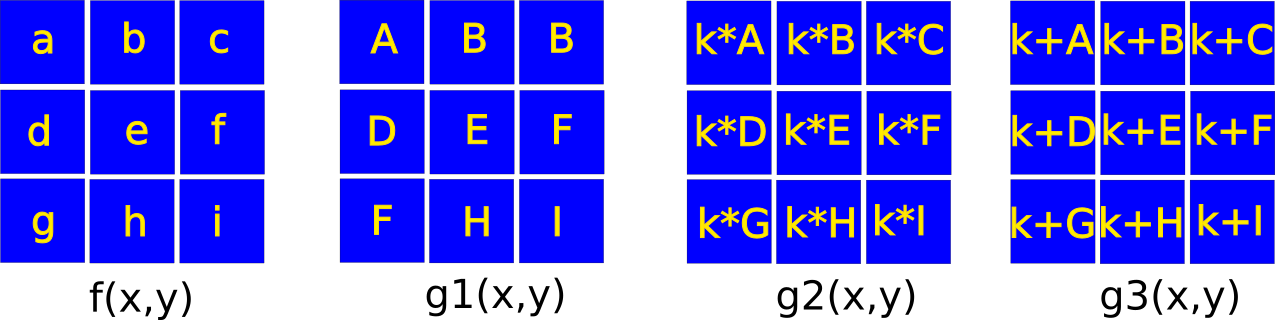
\includegraphics[width=13cm]{correl_const_4.png}
\caption{Correlation with a constant change pixel value patch}
\label{fig:1.1}
\end{figure}
Our correlation and NCC coefficient between $f$ and $g_1$ is:
\begin{equation}
C_{fg_1} = Aa+Bb+Cc+Dd+Ee+Ff+Gg+Hh+Ii
\end{equation}
\begin{equation}
NCC_{fg_1} = \frac{Aa+Bb+Cc+Dd+Ee+Ff+Gg+Hh+Ii}
				  {\sqrt{(A^2+B^2+C^2+D^2+E^2+F^2+G^2+H^2+I^2)*(a^2+b^2+c^2+d^2+e^2+f^2+g^2+h^2+i^2)}}
\end{equation}

Our correlation and NCC coefficient between $f$ and $g_2$ is:
\begin{equation}
C_{fg_2} = k*(Aa+Bb+Cc+Dd+Ee+Ff+Gg+Hh+Ii)
\end{equation}
\begin{equation}
NCC_{fg_2} = \frac{k*(Aa+Bb+Cc+Dd+Ee+Ff+Gg+Hh+Ii)}
				  {\sqrt{k^2(A^2+B^2+C^2+D^2+E^2+F^2+G^2+H^2+I^2)*(a^2+b^2+c^2+d^2+e^2+f^2+g^2+h^2+i^2)}}
\end{equation}

So, the correlation coefficient is varies with constant illumination change if we compute with correlation (eq \ref{eq:1.2} gives $C_{fg_2} =k*C_{fg_1}$), but it rests equal if we take NCC value (eq \ref{eq:1.3} gives $NCC_{fg_2} = NCC_{fg_1}$). 

But, if the changement of intensity value is a shifted constant value on the whole image patch, like from $g_1(x,y)$ to $g_3(x,y)$ (Figure \ref{fig:1.1}), both correlation and NCC value is varies also. To minimize the effect of this problem on correlation score, we normalize each pixel intensity and image patch standard deviation value with the image patch mean intensity value before compute correlation:

\begin{equation}
ZNCC_{fg} = \frac{\sum_{i=1}^{N}\sum_{j=1}^{M}(f(x_i,y_j)-\bar{f})*(g(x_i,y_j)-\bar{g})}
{\sqrt{\sum_{i=1}^{N}\sum_{j=1}^{M}(f(x_i,y_j)-\bar{f})^2*\sum_{i=1}^{N}\sum_{j=1}^{M}(g(x_i,y_j)-\bar{g})^2}}
\label{eq:1.8}
\end{equation}

Equation \ref{eq:1.8} called \textit{\textbf{Zero Mean Normalized Cross Correlation}}. It gives value varies in $[0,1]$ with the higher is the better correlate.

\section{Implementation in MicMac} 
We try to implemented in MicMac a little program that find a best matched position of a little template (image patch) in a large target image. 

Our very simple test describe below:
\begin{itemize}
  \item Take an image (target)
  \item Cut an image patch, use it as a matching template.
  \item We try to re-find the position of image patch in taget.
\end{itemize}

\begin{figure}[h] 
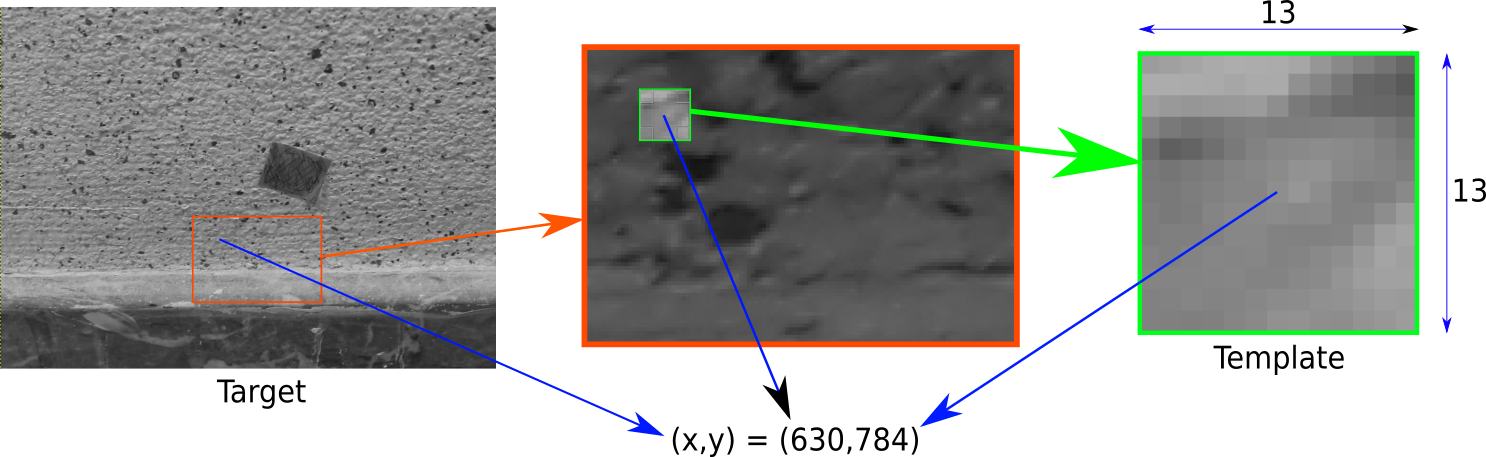
\includegraphics[width=15cm]{template_target.png}
\caption{Template taken from image (target) and ground truth position}
\label{fig:1.2}
\end{figure}

The program is implemented in \textit{"micmac/src/TpMMPD/Ex\_Match"}, 
with command \textit{"mm3d TestLib LSQMatch"}. 
\subsection{Using class RMat\_Inertie}
The correlation compute part is written in {\color{blue}cLSQTemplate.cpp} with 2 sub function:
\begin{itemize}
	\item {\color{blue}dblTst\_Correl1Win}: compute correlation score between 2 image patch.
	\item {\color{blue}dblTst\_Correl}: search for best matched position between template image patch and target image by compute correlation score for template image patch with all position in target image, by calling {\color{blue}dblTst\_Correl1Win}.
\end{itemize}
\begin{lstlisting}
double dblTst_Correl1Win
    (
     tIm2DM & Im1,      	// image 1
     const Pt2dr & aP1,		// center coordinate of image patch 1
     tIm2DM & Im2,	  		// image 2
     const Pt2dr & aP2,		// center coordinate of image patch 2
     const Pt2dr   aSzW,	// size of correlation windows
     const int aStepPxl,	// pixel sampling step
     const cInterpolateurIm2D<double> & aInterPol	//an interpolater
    )
{
    /* Compute point most up & most down for two images patch
     * check if we can take the patch with coordinate and windows size given
     */
    Pt2dr aPtSupIm1 = aP1 + aSzW;
    Pt2dr aPtInfIm1 = aP1 - aSzW;
    Pt2dr aPtSupIm2 = aP2 + aSzW;
    Pt2dr aPtInfIm2 = aP2 - aSzW;
    // if one of these point lie outside the image => quit program
    if (!(
            (InsideREAL(Im1, aPtSupIm1) && InsideREAL(Im1, aPtInfIm1))
            &&
            (InsideREAL(Im2, aPtSupIm2) && InsideREAL(Im2, aPtInfIm2))
       ) )
            return (TT_DefCorrel);
            
     double aDefInter = -1.0; // default value for interpolater
     Pt2dr aVois;
     RMat_Inertie aMatr;

     for  (aVois.x = -aSzW.x ; aVois.x<=aSzW.x  ; aVois.x = aVois.x+aStepPxl)
     {
          for  (aVois.y = -aSzW.y ; aVois.y<=aSzW.y  ; aVois.y = aVois.y+aStepPxl)
          {
              // get pair of pixel in 2 image patch and add them to RMat_Inertie
               Pt2di aPtIm1 = Pt2di(aP1+aVois);         
               aMatr.add_pt_en_place
               (
                 Im1.GetR(aPtIm1),  // get pixel in image patch 1
                 Im2.Get(aP2+aVois, aInterPol, aDefInter)  // get pixel in image patch 2
               );
          }
     }
	 // Compute correlation value
     return aMatr.correlation();
}
\end{lstlisting}
\begin{lstlisting}
cResulRechCorrel dblTst_Correl
 (
  tIm2DM & Im1,         // image 1
  const Pt2dr & aP1,    // center coordinate of image patch 1
  tIm2DM & Im2,         // image 2
  const Pt2dr & aP2,    // center coordinate of search zone on image 2
  const Pt2dr aSzW,     // size of correlation windows
  const double   aStep, // correlation windows movement step
  const int   aStepPxl, // correlation pixel sampling step
  const Pt2dr   aSzRech,// size of search zone
  tIm2DM & ImScore,     // score correlation image (result)
  const cInterpolateurIm2D<double> & aInterPol, // interpolator for pixel sampling
  bool & OK             // if everythings is ok
 )
{
    /* Compute point most up & most down for two images patch
     * check if we can take the patch with coordinate and windows size given
     */
    Pt2dr aPtSupIm1 = aP1 + aSzW;
    Pt2dr aPtInfIm1 = aP1 - aSzW;
    // taken in account some reserve for interpolater
    int aSzInterpol = aInterPol.SzKernel();
    Pt2dr aPtSupIm2 = aP2 + aSzRech + Pt2dr(aSzInterpol, aSzInterpol);
    Pt2dr aPtInfIm2 = aP2 - aSzRech - Pt2dr(aSzInterpol, aSzInterpol);
    cout<<aPtSupIm1<<aPtInfIm1<<" "<<aPtSupIm2<<aPtInfIm2<<endl;
    if (!(
            (InsideREAL(Im1, aPtSupIm1) && InsideREAL(Im1, aPtInfIm1))
            &&
            (InsideREAL(Im2, aPtSupIm2) && InsideREAL(Im2, aPtInfIm2))
       ) )
    {
            OK=false;
            return (cResulRechCorrel (Pt2dr(-1,-1),TT_DefCorrel));
    }
	
    double aScoreMax = -1e30;
    Pt2dr  aDecMax;
    Pt2dr  aP;
    // sweep the correlation windows over image 2
    for (aP.x=-aSzRech.x ; aP.x<= aSzRech.x ; aP.x = aP.x + aStep)
    {
        for (aP.y=-aSzRech.y ; aP.y<= aSzRech.y ; aP.y = aP.y + aStep)
        {
             // compute correlation score 
             double a2Sol  = dblTst_Correl1Win(Im1,aP1,Im2,aP2+aP,aSzW,aStepPxl,aInterPol);
             if (a2Sol > aScoreMax)
             {
                 // update max score and best matched position
                 aScoreMax = a2Sol;
                 aDecMax = aP;
             }
             // write correlation score value in result image
             ImScore.SetR_SVP(Pt2di(aP2 + aP),a2Sol);
        }
     }
     OK = true;
     return cResulRechCorrel(Pt2dr(aP2+aDecMax),aScoreMax);
}
\end{lstlisting}

Let see how the class {\color{blue}RMat\_Inertie} compute correlation score. This class is created from class {\color{blue}Mat\_Inertie} with value type {\color{blue}double}. Class is defined and implemented in \textit{"micmac/include/general/geom\_vecteur.h"}. 
\begin{lstlisting}
/*
 * class variable member and constructor
 */
Mat_Inertie
 (
  ElTyName Type::TypeScal S,
  ElTyName Type::TypeEff  S1,
  ElTyName Type::TypeEff  S2,
  ElTyName Type::TypeScal S11,
  ElTyName Type::TypeScal S12,
  ElTyName Type::TypeScal S22
 )
 :
  _s     (S),	// _s: number of pixel pair added
  _s1    (S1),  // _s1: sum of all (v1), with v1 is intensity value of pixel image 1
  _s2    (S2),  // _s2: sum of all (v2), with v2 is intensity value of pixel image 2
  _s11   (S11), // _s11: sum of all (v1)*(v1)  => standard deviation of img 1
  _s12   (S12), // _s11: sum of all (v1)*(v2)
  _s22   (S22)  // _s22: sum of all (v2)*(v2)  => standard deviation of img 2
  {
  }

/* Pre-compute needed value for each pixel pair added  */ 
void add_pt_en_place(ElTyName Type::TypeEff v1,ElTyName  Type::TypeEff v2)
       {
            _s   += 1;	// increase counter of number of pixel pair added
            _s1  += v1;
            _s2  += v2;
            _s11 += scal(v1,v1);  // scal (v1,v1)=(v1)*(v1)
            _s12 += scal(v1,v2);
            _s22 += scal(v2,v2);
       }

/* Normalize pixel value */   
Mat_Inertie<ElTyName Type::TypeReel>  normalize() const
       {
       // check if there are pixel to normalize
             ELISE_ASSERT
             (
                  _s != 0,
                  "som pds = 0 in Mat_Inertie::normalize"
             );

             ElTyName Type::TypeReel::TypeEff  S1 =  _s1 / (REAL) _s;  
             ElTyName Type::TypeReel::TypeEff  S2 =  _s2 / (REAL) _s;  


#if ( ELISE_windows & ELISE_MinGW )
    return Mat_Inertie<typename Type::TypeReel>
#else
    return Mat_Inertie<ElTypeName_NotMSW Type::TypeReel>
#endif
                    (
                         _s,
                         S1,	// => sigma(v1)/_s = moyen(v1)
                         S2,    // => sigma(v2)/_s = moyen(v2)
                         _s11/(REAL)_s  -scal(S1,S1),  // =>   
                         _s12/(REAL)_s  -scal(S1,S2),
                         _s22/(REAL)_s  -scal(S2,S2)
                    );
       }
\end{lstlisting}
\begin{lstlisting}
/* Compute ZNCC correlation score*/
REAL  correlation(REAL epsilon = 1e-14) const
       {
           #if ( ELISE_windows & ELISE_MinGW )
           /* Normalize pixel value */
             Mat_Inertie<typename  Type::TypeReel> m =  normalize();
           #else
             Mat_Inertie<ElTypeName_NotMSW  Type::TypeReel> m =  normalize();
           #endif
             return m.s12() / sqrt(ElMax(epsilon,m.s11()*m.s22()));
       }

\end{lstlisting}


\subsection{Using class cCorrelImage}
This is another class use to compute correlation score also (Jean-Michael Muller).
In this class, the implementation idea is 1 object of this class is 1 image patch.
Have a look at class declaration: 

\begin{lstlisting}
/* Idea General: 1 object of this class is 1 image patch */
class cCorrelImage
{
  public :
    cCorrelImage();
    /* Im2D and TIm2D is 2 image type usually use in MicMac.
     * The different ?Hmmmm....TIm2D let pixel access faster in some case...
     * But TIm2D can declare from an Im2D object.
     * So, we will usually see these 2 type comes together
     */
    Im2D<U_INT1,INT4> * getIm(){return &mIm;}
    TIm2D<U_INT1,INT4> * getImT(){return &mTIm;}
    // compute correlation coeff between this image patch & aIm2 image patch
    double CrossCorrelation(const cCorrelImage & aIm2);
    /* compute covariance b/w this image patch & aIm2 image patch:
     * cov = sigma(f*g)/(sqrt(1+2n))     
     */
    double Covariance(const cCorrelImage & aIm2);
    // mSzW => half size of correlation windows
    int getSzW();
    // mSz => size of correlation windows
    Pt2di getmSz();
    /* extract image patch with size = mSz at position (aCenterX, aCenterY) 
     * from a large image anIm
     */
    void getFromIm(Im2D<U_INT1,INT4> * anIm,double aCenterX,double aCenterY);
    // copy whole image anIm as image patch
    void getWholeIm(Im2D<U_INT1,INT4> * anIm);
    // Set size for correlation windows
    static void setSzW(int aSzW);
    static int mSzW;

  protected:
    // pre-compute value needed for correlation => compute mImS1 & mImS2
    void prepare();
    Pt2di mSz;
    //this image patch in 2 types Im2D & TIm2D
    TIm2D<U_INT1,INT4> mTIm; 
    Im2D<U_INT1,INT4>  mIm;
    // each pixel in mIm with their value v1 becomes v1/(1+2n)
    TIm2D<REAL4,REAL8> mTImS1; 
    Im2D<REAL4,REAL8>  mImS1;
    // each pixel in mIm with their value v1 becomes (v1)^2/(1+2n)
    TIm2D<REAL4,REAL8> mTImS2; 
    Im2D<REAL4,REAL8>  mImS2;
};
\end{lstlisting}

To use this class, a litte code is written in {\color{blue}cLSQTemplate.cpp}, in {\color{blue}"main"} function, part "Corrrelation by cCorrelImage". Let see and explication how to use it:
\begin{lstlisting}
typedef Im2D<unsigned char, int> tIm2DcCorrel;
typedef TIm2D<unsigned char, int> tTIm2DcCorrel;
// cResulRechCorrel just for contain correlation result (coordinate & score)
cResulRechCorrel aResCorrel(Pt2dr(-1,-1),TT_DefCorrel);
// create correlation result image
tIm2DM aImgScoreCorrel(aImgTarget->Im2D().sz().x, aImgTarget->Im2D().sz().y);
// Load Image to type Im2D<unsigned int, int> => class cCorrelImage require this image type
Pt2di aSzImTarget = aImgTarget->Im2D().sz();
Pt2di aSzImTmp = aImgTmplt->Im2D().sz();
tIm2DcCorrel aCImTmpl(aSzImTmp.x, aSzImTmp.y);
tIm2DcCorrel aCImTarget(aSzImTarget.x, aSzImTarget.y);
ELISE_COPY(aCImTmpl.all_pts(), aImgTmplt->Tif().in(), aCImTmpl.out());
ELISE_COPY(aCImTarget.all_pts(), aImgTarget->Tif().in(), aCImTarget.out());
/* 
 * At this moment, we have loaded a template image patch aCImTmpl
 * and a full target image aCImTarget, with the type used for class cCorrelImage.
 * Now, we will create a template image patch as object of class cCorrelImage,
 * and scan through target image aCImTarget, creat a target image patch as object   
 * of class cCorrelImage to compute correlation score at each position.
 */

// Before using cCorrelImage class, we need to set image patch size (half size)
cCorrelImage::setSzW(aSzW.x);  
// Now, when we create a new image patch object, it will initialize with size = aSzW*2+1
cCorrelImage ImPatchTmpl;
// Take all template image as template image patch
ImPatchTmpl.getWholeIm(&aCImTmpl);
// Create a target image patch, size aSzW*2+1, for now it's empty
cCorrelImage ImPatchTarget;
bool corOK = false;
Pt2dr aPt(0,0);
OK = true;

         // Now, scan through target image, each pixel position:
         for (aPt.x=0; aPt.x<aSzImTarget.x; aPt.x = aPt.x + (int)aParam.mStepCorrel)       
         {
             for (aPt.y=0; aPt.y<aSzImTarget.y; aPt.y = aPt.y + (int)aParam.mStepCorrel)
             {
                 Pt2dr aPtInf = aPt-Pt2dr(ImPatchTmpl.getmSz());
                 // if image patch is inside image
                 if (    (aPtInf.x >= 0 && aPtInf.y >= 0)
                      && (aPtInf.x < aSzImTarget.x && aPtInf.y < aSzImTarget.y) )
                 {
                      // Load image patch at position aPt from target image
                      ImPatchTarget.getFromIm(&aCImTarget, aPt.x, aPt.y);
                      // compute correlation score b/w 2 image patch
                      double aScore = ImPatchTmpl.CrossCorrelation(ImPatchTarget);
                      corOK = true;
                      if (aScore > aResCorrel.mCorrel)
                      {
                      	  // update best match position
                          aResCorrel.mCorrel = aScore;
                          aResCorrel.mPt = Pt2dr(aPt);
                      }
                      // write score to correlation result image
                      aImgScoreCorrel.SetR_SVP(Pt2di(aPt), aScore);
                 }
                 else
                 {
                      corOK = false;
                      aImgScoreCorrel.SetR_SVP(Pt2di(aPt),-1.0);
                 }
             }
         }
}
if (OK)
   cout<<"Correl : "<<aResCorrel.mCorrel<<" - Pt: "<<aResCorrel.mPt<<endl;
else
    cout<<"Correl false"<<endl;
\end{lstlisting}

Execute command that implemente this example:
\begin{verbatim}
mm3d TestLib LSQMatch Temp_13_Test.png Target.png StepCor=1 NbIter=0 Meth=1
\end{verbatim}
Params: "StepCor=1" is the movement step of correlation windows. "Meth=1" to tell the program compute correlation by class {\color{blue}cCorrelImage}. We obtain result:
\begin{verbatim}
Correl : 0.99999 - Pt: [630,784]
\end{verbatim}
which is exact match (view ground truth and dataset in Figure \ref{fig:1.2})

\subsection{Using class Optim2DParam}

\subsection{CENCUS}
Function CencusBasic, CencusBasicCenter (regarder Param XML\_MICMAC.xml, search Cencus), 

MutualInformation (pas dans micmac): Similarity=(Entropy(g) *entropy(f))/(Entropy(g*f))


\end{document}
